

\begin{flushleft}

	
{\color{Blue}{\subsection{Overview}}}
Both Data4Help ad AutomatedSOS are complex services due to the large set of technologies involved in their functionalities. To have a full comprehension of the overall architecture, it is necessary to abstract the entire system, starting the analysis from the customer perspective. Here, in fact, the main challenge is related to device management and data representation, since a large variety of sensors (supported by the service), can be connected and send data simultaneously. Each health indicator sample provided to the app should be processed at first in order to match a common data structure and then sent to the server. Since a D4H user is automatically an ASOS user (once the first login is performed), it may happen that both applicationswill be used in tandem. This leads to a problem of data redundancy, since the server could receive two samples from the same monitoring device. It has been chosen to avoid either the effort foo the server to analyze and discard in real time duplicated samples or to store identical dataset parts in the database system: as anticipated in the introduction, both the services provided by TrackMe for several reasons will rely on the same dataset for each monitored user. The solution to the mentioned problem is based on a messaging system operating between the apps and the server to synchronize the monitoring sessions and avoid any conflict. The mechanism will be discussed later.\\
Since client and server architectures are characterized by some different aspects and responsibilities, both of them will be defined and carefully analyzed in this document. An high level view of the entire system, anyway, can be provided by the following picture:

\begin{figure}[H]
	\centering
	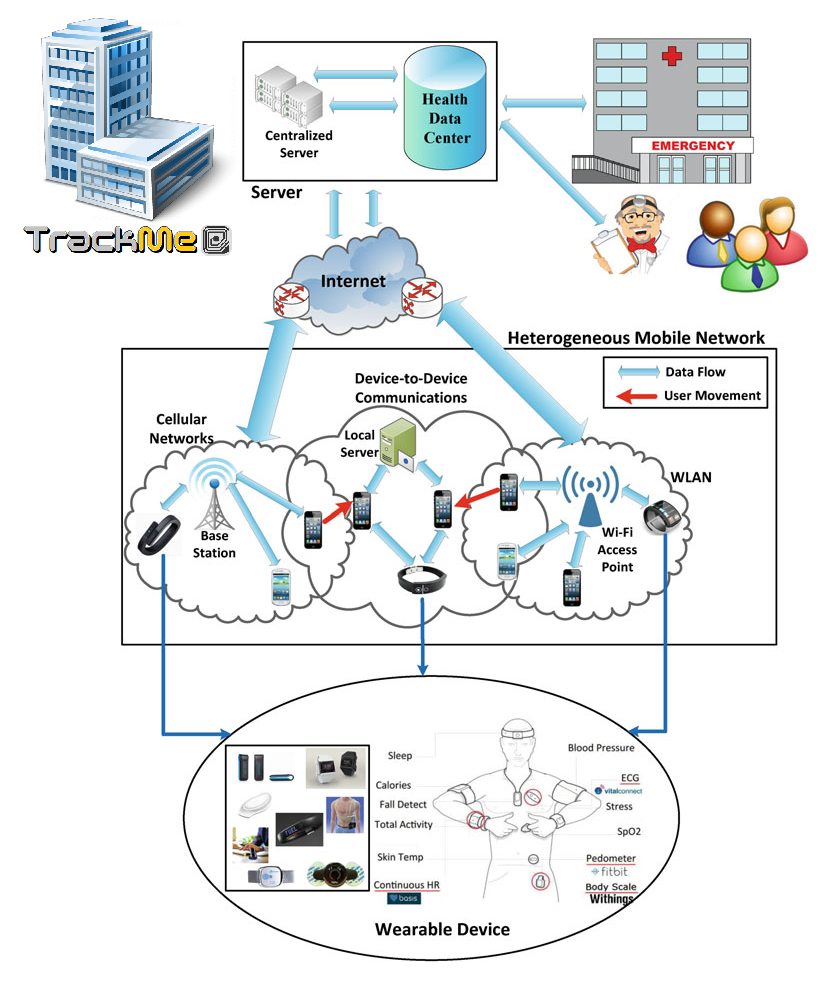
\includegraphics[scale=0.7]{images/system_perspective}
	\caption{High-level View of the System}
	\label{Figure 1}
\end{figure}
\newpage

{\color{Blue}{\subsection{Component View}}}
{\setlength{\parskip}{0.3cm}
In this section is provided a brief description of the common components in D4H and ASOS apps for what concerns hardware interaction and about the mechanism that regulates the messages and data exchange between the client and the server. In the analysis of server-side architecture in subsection \textit{2.2.4}, the component view has been splitted in two parts in order to help the comprehension of the way the architecture works. The first part is related to user data collection and health status observation, the second one presents the functionalities that deal mostly with Data4Help mansions (device and third party request management, privacy and security constraint evaluator and so on).

{\color{Blue}{\subsubsection{Common Components}}}

Starting from the client-side architecture, there are common aspects between the two applications for what concerns the hardware interaction part and activity synchronization. Respectively, in the first case the system provides:
\begin{itemize}
	\item \textbf{DeviceProxy:} a software interface for the control of each specific device. It implements different methods to directly interact through the proper API with the real device. It encapsulates also all the essential information about the smart sensor;
	\item \textbf{DeviceManager:} that handles with all the connected devices. It is in charge of:
	\begin{itemize}
		\item instantiate a device when it is required;
		\item activate and deactivate a single device when an event occurs; 
		\item give information about the status of the device set.
	\end{itemize}
	\item \textbf{Data Collector:} that implements all the algorithms required to perform data collection according to specific patterns.
\end{itemize}  
For both client and server architectures, in order to synchronize all the activities carried on by the system, a mechanism of message exchange has been designed. This includes:
\begin{itemize}
	\item \textbf{EventObserver:} that mediates the interaction among the manager components (all those components responsible of managing a specific set of functionalities in the system) and the server;
	\item \textbf{EventHandling:} an interface implemented by manager components. It includes the essential methods required to send notifications when a particular event occurs and to perform specific activities when messages are received by other manager components and the server (through the EventObserver).
\end{itemize} 

\newpage
{\color{Blue}{\subsubsection{Data4Help Client Components View}}}
Specifically to Data4Help on client side, the component in addition to the above mentioned is the \textbf{DataRequestManager}, it implements all those basic functionalities that allow the user to receive and evaluate third party requests.

\begin{figure}[H]
	\centering
	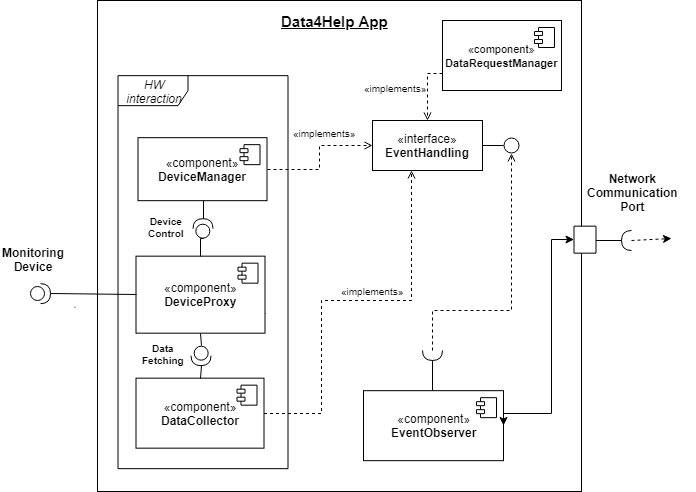
\includegraphics[scale=0.6]{images/uml/D4H_client_component}
	\caption{D4H Client App, Component Diagram}
	\label{Figure 2}
\end{figure}
\newpage

{\color{Blue}{\subsubsection{AutomatedSOS Client Component View}}}
The ASOS application is characterized in addition by:
\begin{itemize}
	\item \textbf{UserHealthProfileManager:} that implements all those operations required to create and modify a health profile for the user. It is a basic component, the information provided by the patient is requested by the server to understand which health parameters to watch over;
	\item \textbf{SupervisorRequestManager:} that deals with Supervisor tasks from the client perspective. It is used to keep track of the supervised users or to send, receive and manage external requests of supervision.
\end{itemize}

\begin{figure}[H]
	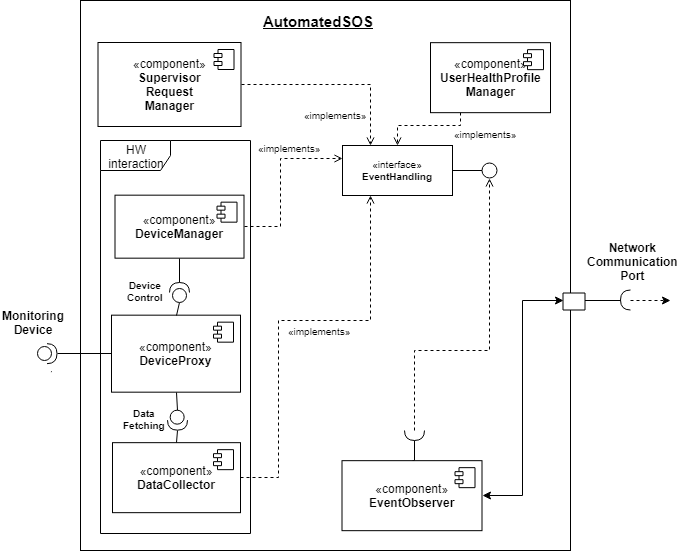
\includegraphics[scale=0.6]{images/uml/ASOS_client_component}
	\caption{ASOS Client App, Component Diagram}
	\label{Figure 3}
\end{figure}

\newpage

{\color{Blue}{\subsubsection{Server Side Component View}}}
From the server perspective the situation is different. The application logic is almost completely deployed in this part of the system. In order to facilitate the comprehension of the architecture, the component diagram has been splitted.\\
As said, Data4Help and AutomatedSOS performs different tasks but they work on the same dataset, so the part that deals with data collection must be considered as common to both the applications that in some other cases will communicate exclusively with specific components.\\
Before describing the architecture it is needed to introduce some key concepts. In particular, the time in which the system collects and provides personal data from user monitoring devices will be divided in intervals, each one called \textit{session}. A session, from server perspective, can be thought as a group of data queues with a proper ID, associated to all the health indicators monitored from a specific user and a data stream directly connected to a component called, Analyzer. Since for real-time requirements ASOS needs to process each received sample as fast as possible, a software component will dispatch a copy of each value in a data stream (at first) and consequently in the proper queue. The Analyzer, in charge of processing data to monitor user condition, will receive data only from the stream. Periodically and according to the frequency of sample arrivals, each queue will be stored in the database.\\
The following high-level diagram clearly represents the described mechanism.

\begin{figure}[H]
	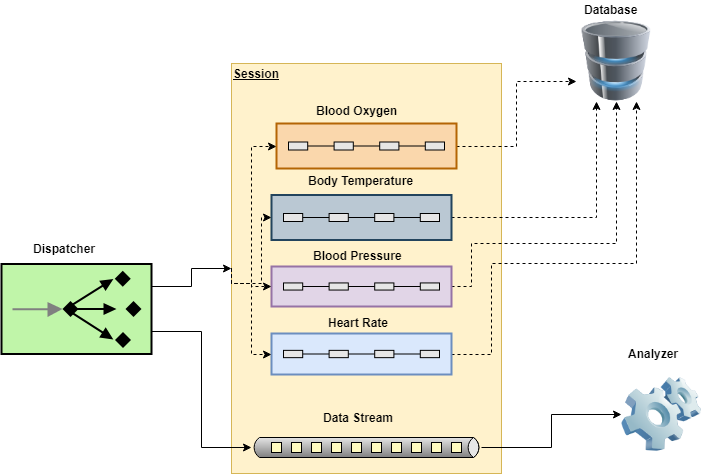
\includegraphics[scale=0.5]{images/uml/server_schema.png}
	\caption{High-level View of Session Management}
	\label{Figure 4}
\end{figure}

Other software artifacts regarding this side of the system are:
\begin{itemize}
	\item \textbf{SessionManager:} that is responsible to create and manage each session. In particular it will handle the situations in which the apps running in tandem will require a context switch for the current session;
	\item \textbf{Analyzer:} one of the most complex parts of the architecture, implements all the algorithms and mechanisms required to process ASOS data stream and establish with appreciable certainty the situation of the user;
	\item \textbf{EmergencyCondition:} that encapsulates all the information regarding a detected urgency (health status, user, location and so on), for which immediate assistance is required;
	\item \textbf{AnomalyCondition:} that encapsulate the mechanisms and information to handle a suspicious state of urgency;
	\item \textbf{SupervisorManager:} in charge of managing supervisor operations at server side;
	\item \textbf{ERMManager:} an interface component that allows the system to communicate with external ERMs;
	\item \textbf{Resource:} a part of the architecture that is used to keep track of the resource status instantiated by the ERM, once dispatched;
	\item \textbf{DatabaseManager:} a common element of both the diagrams, it will provide an interface efficiently implemented to the database system.
\end{itemize}

Here is the first part of the server side component:
\begin{figure}[H]
	\centering
	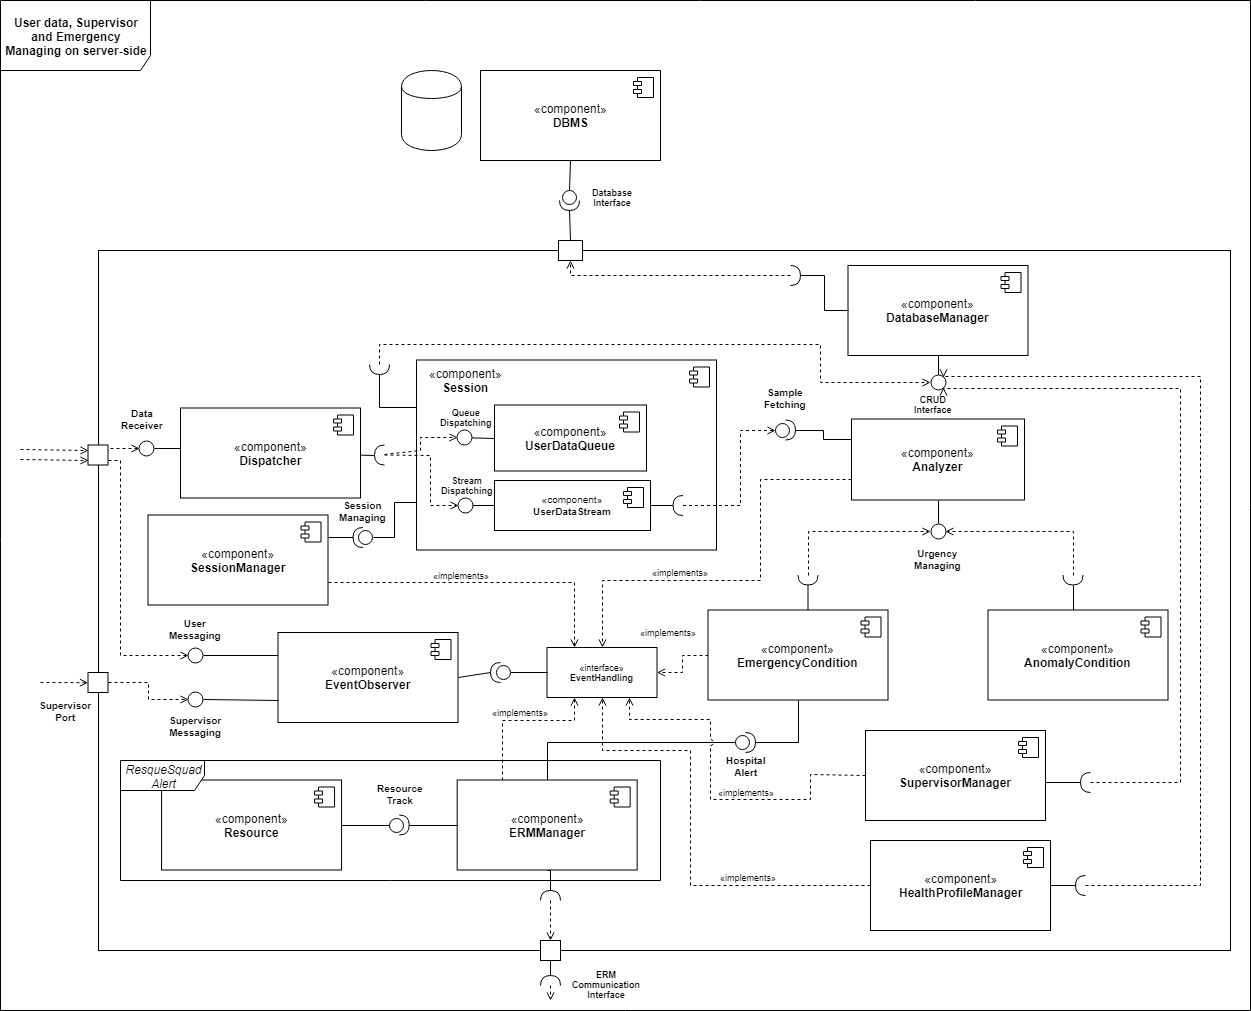
\includegraphics[scale=0.4]{images/uml/ASOS_server_emergency_component}
	\caption{Emergency Handling and User Monitoring on Server Side, Component Diagram}
	\label{Figure 5}
\end{figure}

Of course, both the communication system composed by the EventObserver and the EventHandling and the DatabaseManager should be considered as common components in the two component diagrams.
\newpage

In the following diagram is shown the second part of the server architecture, that is more related to D4H functionalities.\\
It is characterized by:
\begin{itemize}
	\item \textbf{DeviceHandler:} to manage system supported devices (add, remove and modify smart sensors that are supported by the services) and allow users to associate devices to their account through the registration mechanism; 
	\item \textbf{Login:} to authenticate users and third parties;
	\item \textbf{TP\_RequestManager:} to process and manage third party requests from the server perspective. This component encapsulates also the methods required to allow third parties to create and manage all the requests and to allow the target users to receive such requests as soon as they are formulated;
	\item \textbf{PrivacyAndSecurityEvaluator:} to enforce an access control policy to user datasets, checking privacy constraint violations for search criteria specified in anonymous requests and to certificate third party identity and reliability;
	\item \textbf{DatasetGenerator:} to generate anonymous or specific user datasets from evaluated and accepted requests. 
\end{itemize}
\begin{figure}[H]
	\centering
	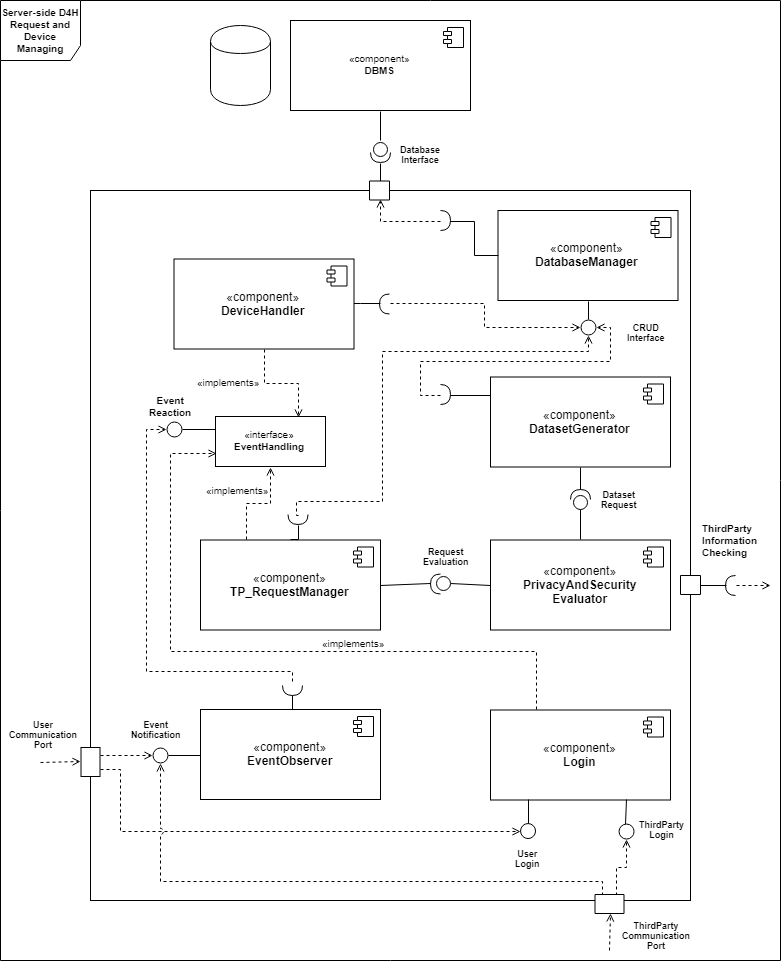
\includegraphics[scale=0.4]{images/uml/D4H_server_requestManaging_component}
	\caption{Device and TP Request Managing on Server Side, Component Diagram}
	\label{Figure 6}
\end{figure}
}
\newpage
As explained before, the reason for event notification through message exchanging between client and server is due to the need to synchronize system activities . A \textbf{Message} can be thought in the design context as an element that generalizes two concepts:
\begin{itemize}
	\item an \textbf{Action}
	\item an \textbf{Event}
\end{itemize} 
The first one is used when an architectural component must communicate a state change to the rest of the system. When the notification needs to be sent to the server, the EventObserver, that is the mediator of each communication, is called by the notifier component (e.g: DeviceManager), it creates a Message and sends it to the server side. When a message is received by the opposite observer, this can be turned either into an Event, if something is required to be communicated to other components, or into an Action, if some operation must be performed. The EventObserver establishes which component is the receiver, calls the method \textit{onReceive} (implemented by each manager component through the interface \textbf{EventHandling}) and passes as parameter an Action. In any case, all these elements are characterized by the same format:

\begin{figure}[H]
	\centering
	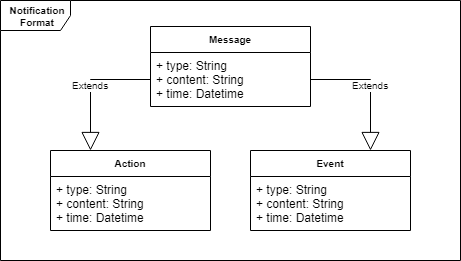
\includegraphics[scale=0.5]{images/uml/message_format.png}
	\caption{Notification Format}
	\label{Figure 7}
\end{figure}

The \textit{type} is used by the EventObserver to understand which is the message receiver, the \textit{content}, to establish which is the operation that the specific component must perform after being notified and the \textit{time} should be used for further implementation of a time scheduling functionality for such component.\\
In many case this mechanism can be useful:
\begin{itemize}
	\item When a user triggers a conflict event such as:
	\begin{itemize}
		\item He/She turns on ASOS when Data4Help is running. In this case the current session is suspended to allow the system to change the context (stream some health parameters used by D4H to the analyzer), notifying the need to switch off some devices in the D4H app in order to not transmit sample copies;
		\item He/She attempts to register/unregister devices when ASOS Monitor Mode is switched on. In this case the server should avoid this condition in order to not raise unexpected conflicts. A warning must be shown to the client;
		\item He/She tries to change the own health profile while ASOS is running in MonitorMode.
	\end{itemize}
	\item During normal activities, such as:
	\begin{itemize}
		\item Register/Unregister a device;
		\item Notify a decision on a specific request (ThirdParty/Supervisor);
		\item Notify changes in health profile;
		\item Notify emergency communication (from both the parts);
		\item Other notifications.
	\end{itemize} 
\end{itemize}

\newpage
{\color{Blue}{\subsubsection{Entity-Relationship Diagram}}}
The following diagram represents the database model of the defined architecture:
\begin{figure}[H]
	\centering
	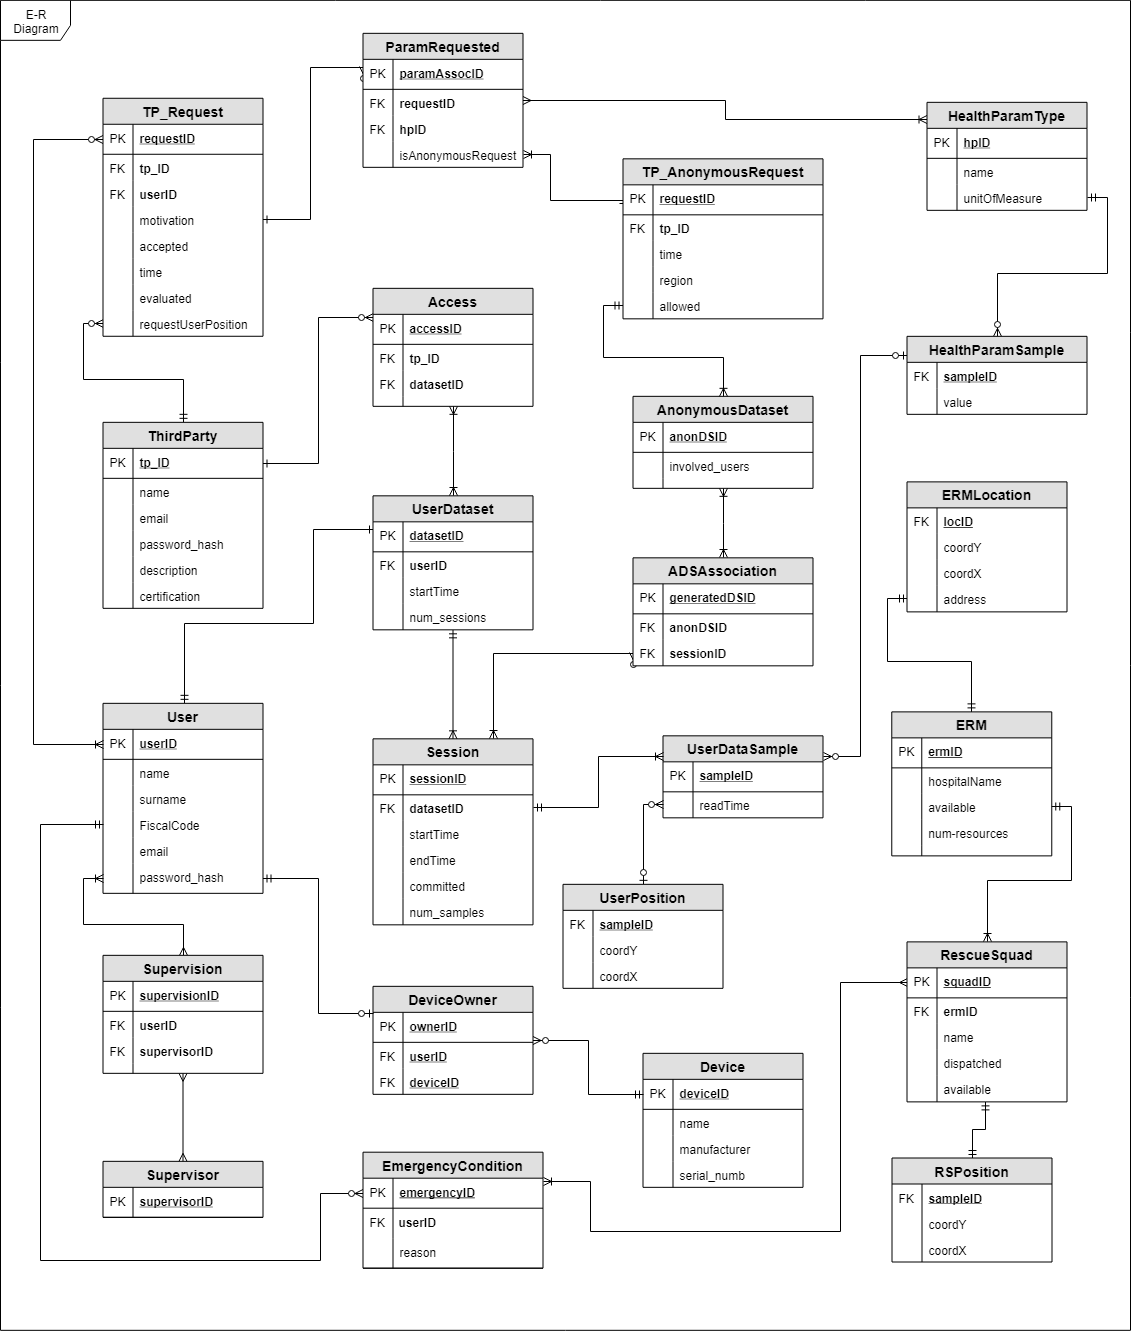
\includegraphics[scale=0.4]{images/uml/ER_diagram.png}
	\caption{E-R Diagram for Database Modeling}
	\label{Figure 8}
\end{figure}


\newpage
{\color{Blue}{\subsection{Deployment View}}}
The deployment diagram represents the displacement of all the physical components involved in the system, how the application logic is inserted in relative execution environments and the communication with the external services (ERM system and ThirdParty database). \\
In the entire system deployment, the following components are involved:
\begin{itemize}
	\item \textbf{Application tier:} in which the system artifacts interact among them in their respective execution environments, in particular:
	\begin{itemize}
		\item \textbf{Data4Help} and \textbf{AutomatedSOS}: that interacts with the application server, by data and message exchange using HTTP over TLS;
		\item \textbf{ThirdParty Web-Browser:} used to allow companies and organizations to access the server logic in order to formulate requests, download datasets, manage their own profile.
	\end{itemize}
	\item \textbf{External Service tier:} composed by the external services with relative APIs and the system logic components required to interact with them, also in this case over an encrypted channel:
	\begin{itemize}
		\item \textbf{ERMSystem:} running on the ERMServer, that is in charge of manage the Rescue Squads (in this document called Resources), it provides the interface required to the ASOS server application to interact with it;
		\item \textbf{ThirdPartyDatabaseServer:} on which the system relies to retrieve information about each company and organization that wants to register or formulate a request to the service.
	\end{itemize}
	\item \textbf{Database tier:} that includes all those logic and physical components used to interface persistent data to the server application (for security reasons through a firewall);
	\item \textbf{SmartSensor:} connected physically to the smartphone using a communication interface such as Bluetooth, BLE, NFC and controlled by the applications through the Android OS.
\end{itemize}

\begin{figure}[H]
	\centering
	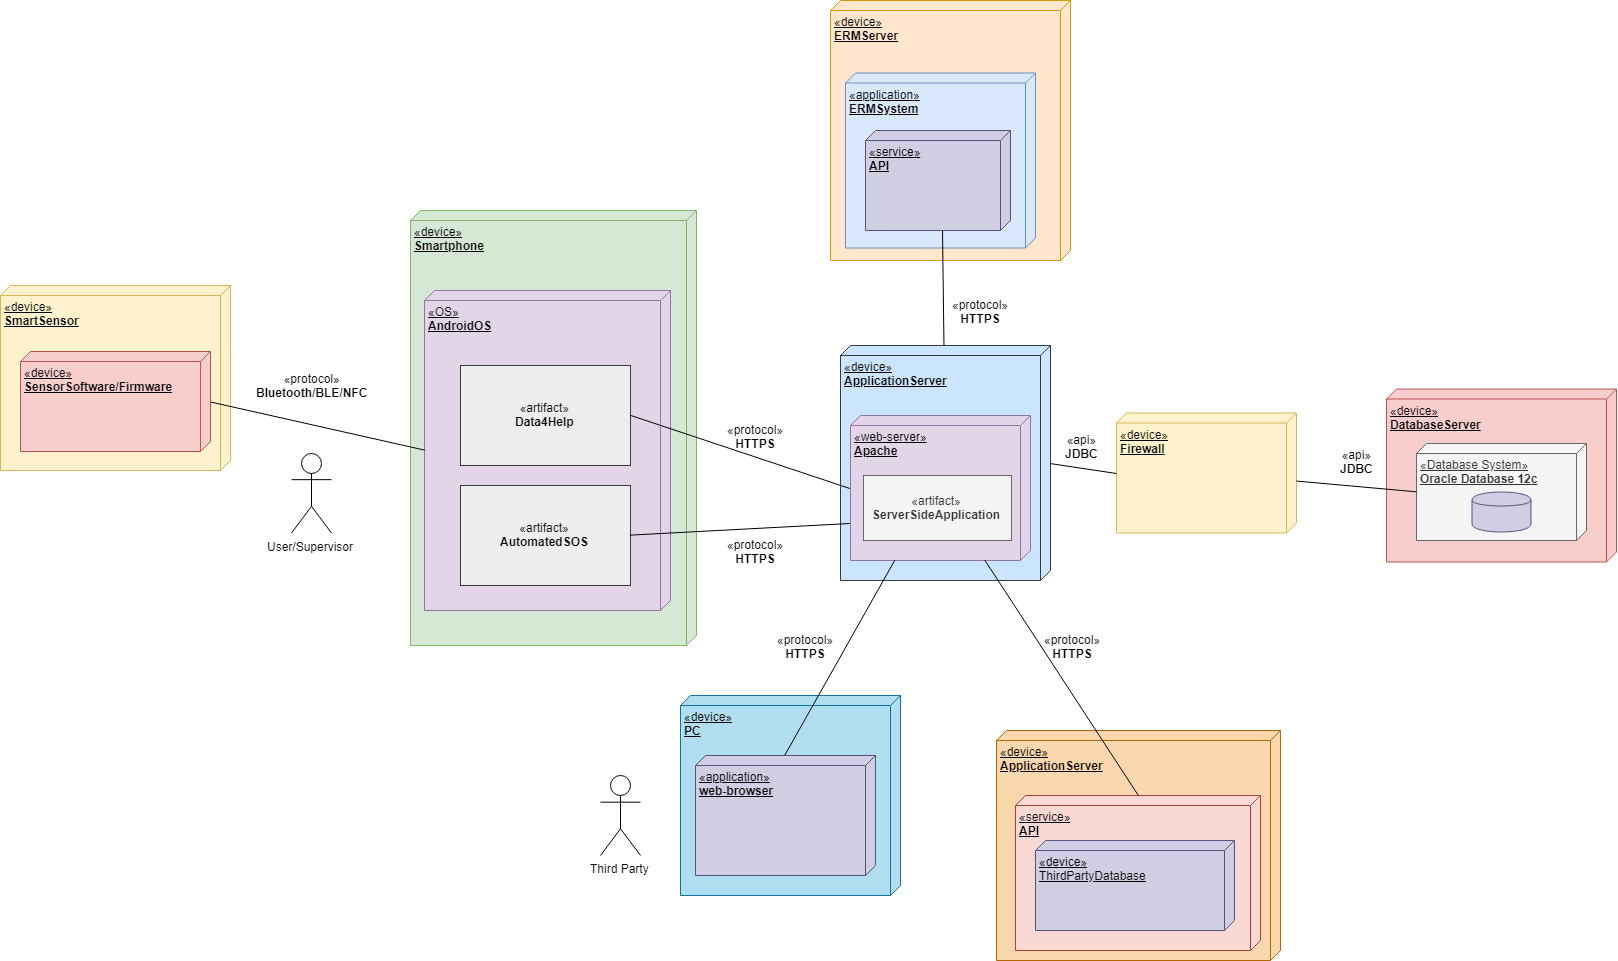
\includegraphics[scale=0.3]{images/uml/deployment}
	\caption{Deployment Diagram}
	\label{Figure 9}
\end{figure}
\newpage

{\color{Blue}{\subsection{Runtime View}}}
The Runtime View provides the interaction sequence for four use cases also mentioned in the RASD document (see \textit{Section 3.5} in the \textit{Requirements Analysis and Specification Document}). No description is provided since the detail level by which the interactions are represented, is enough to understand the event flows.\\

\begin{figure}[H]
	\rotatebox{90}{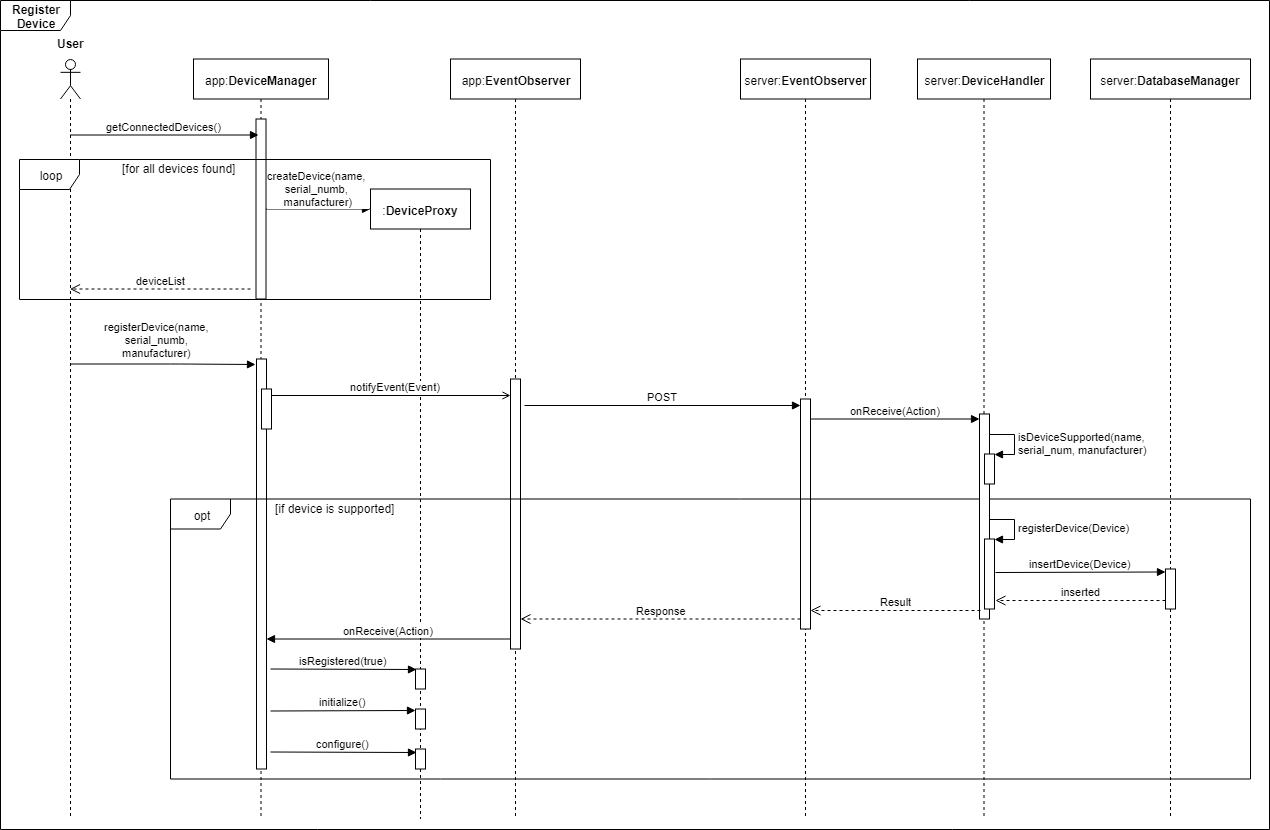
\includegraphics[scale=0.45]{images/uml/D4H_ASOS_device_sequence.png}}
	\caption{Register Device, Sequence Diagram}
	\label{Figure 10}
\end{figure}

\newpage

\begin{figure}[H]
	\rotatebox{90}{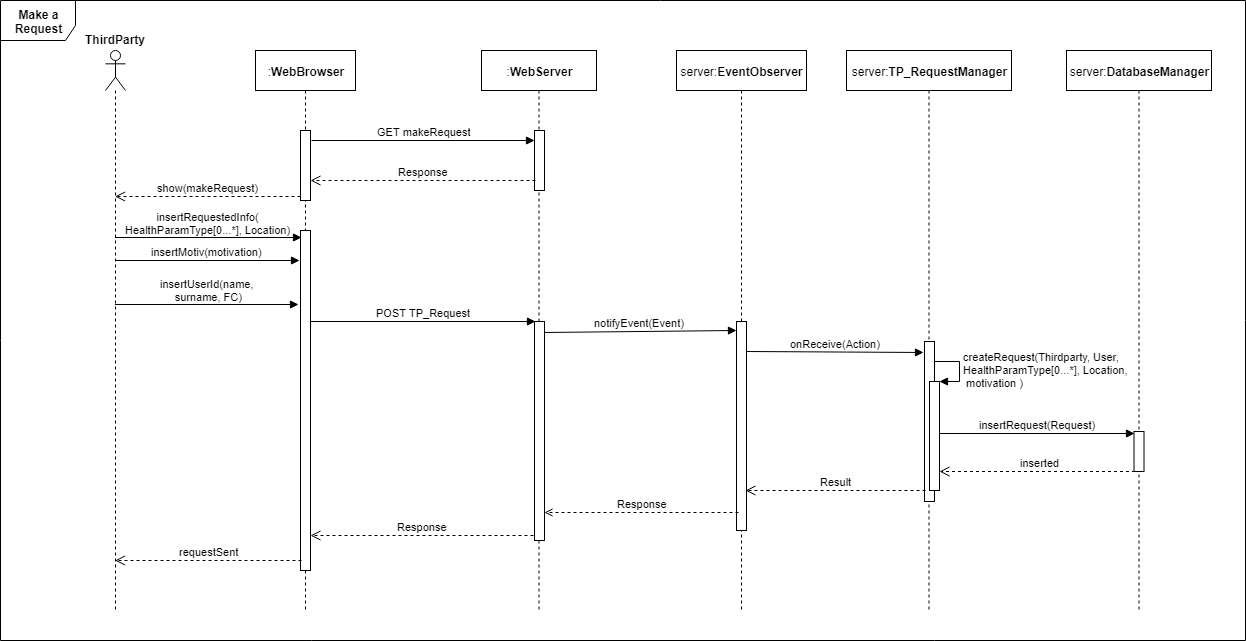
\includegraphics[scale=0.54]{images/uml/D4H_ASOS_makeRequest_sequence.png}}
	\caption{Make a Request, Sequence Diagram}
	\label{Figure 11}
\end{figure}

\newpage

\begin{figure}[H]
	\rotatebox{90}{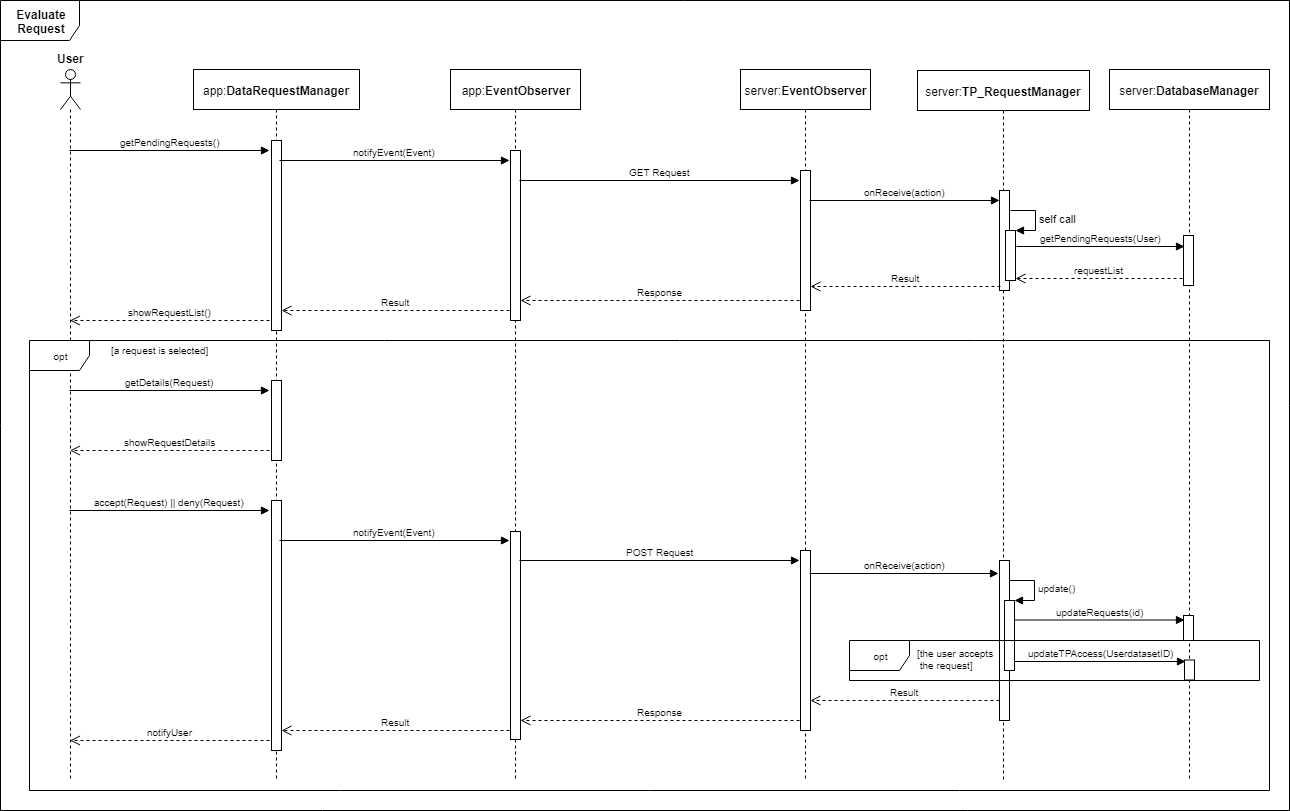
\includegraphics[scale=0.52]{images/uml/D4H_ASOS_evaluateRequest_sequence.png}}
	\caption{Evaluate a Request, Sequence Diagram}
	\label{Figure 12}
\end{figure}

\newpage

\begin{figure}[H]
	\rotatebox{90}{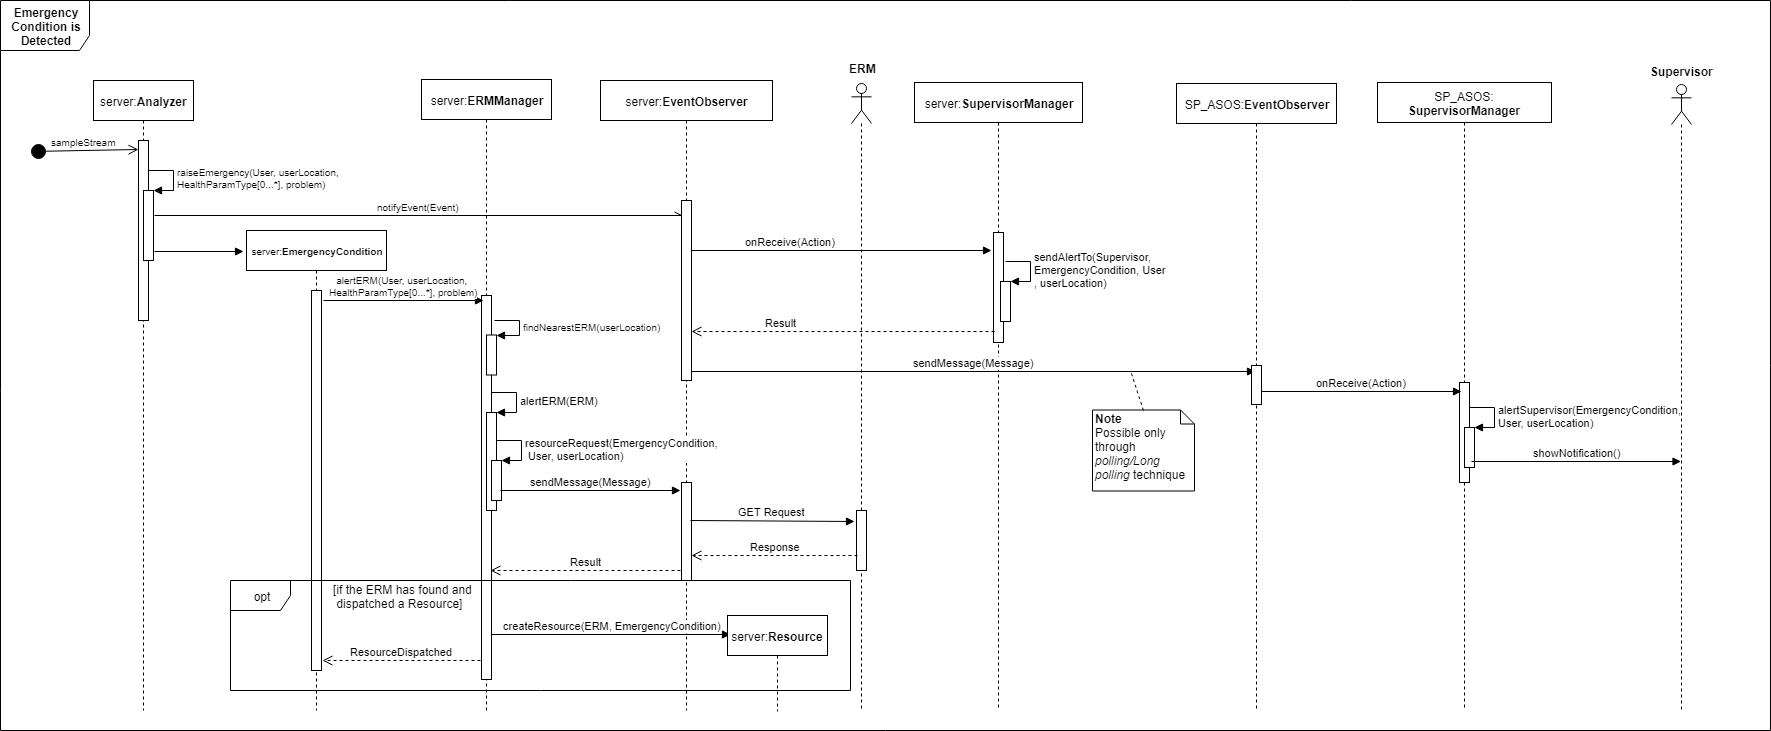
\includegraphics[scale=0.37]{images/uml/D4H_ASOS_Emergency_sequence.png}}
	\caption{Emergency Condition, Sequence Diagram}
	\label{Figure 13}
\end{figure}



{\color{Blue}{\subsection{Component Interfaces}}}
{\setlength{\parskip}{0.3cm}
This section highlights the dependencies among the various interfaces in the system. As in the previous case, it has been made for both client and server architectures.

{\color{Blue}{\subsubsection{D4H Client Component Interfaces}}}
\begin{figure}[H]
	\centering
	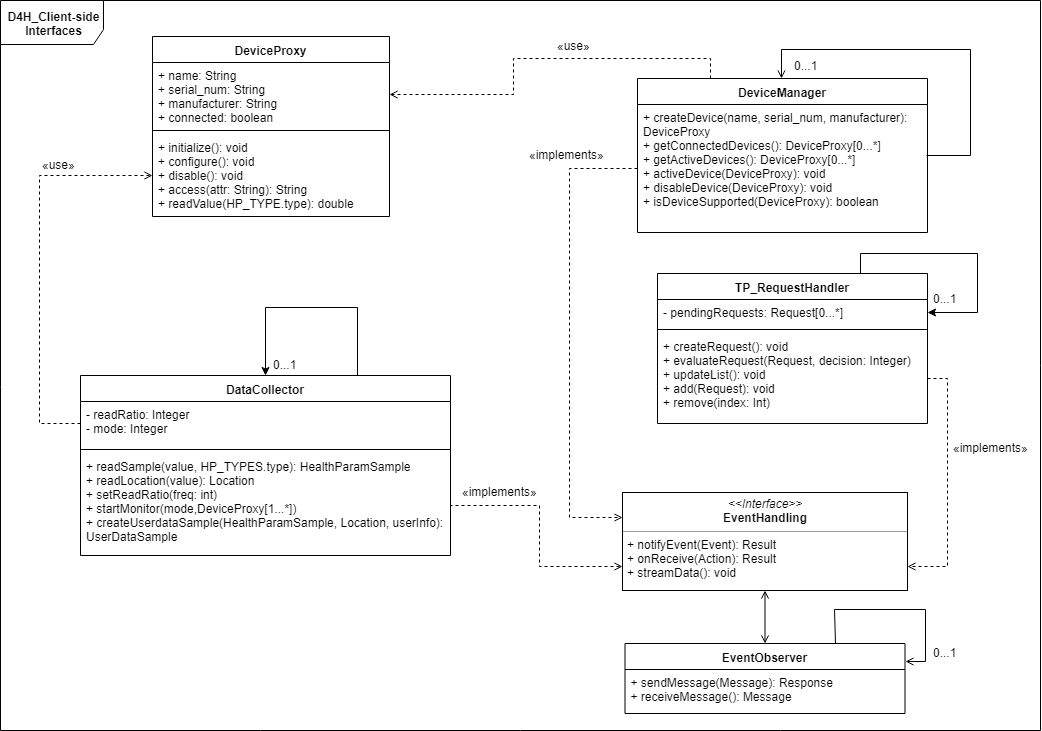
\includegraphics[scale=0.3]{images/uml/D4H_client_interfaces}
	\caption{D4H Client App, Interface Dependencies}
	\label{Figure 14}
\end{figure}


{\color{Blue}{\subsubsection{ASOS Client Component Interfaces}}}


\begin{figure}[H]
	\centering
	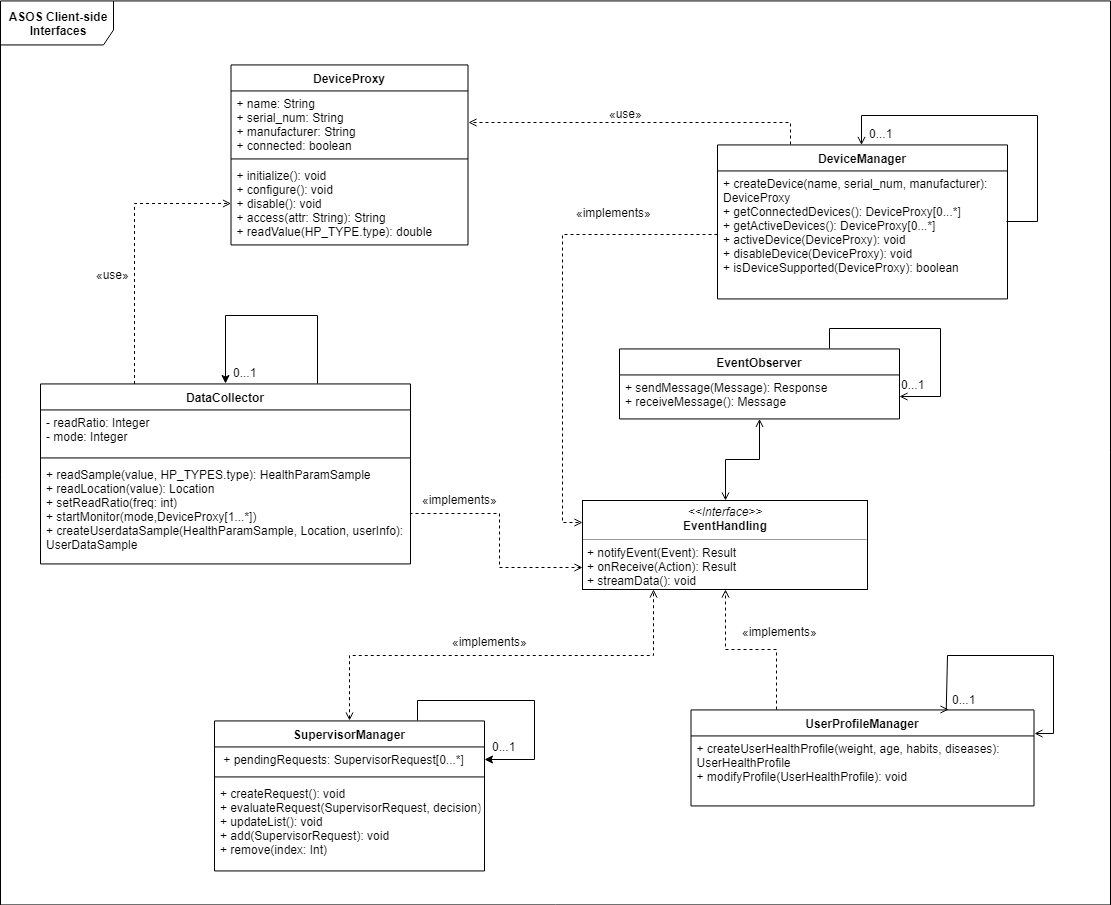
\includegraphics[scale=0.28]{images/uml/ASOS_client_interfaces}
	\caption{ASOS Client App, Interface Dependencies}
	\label{Figure 15}
\end{figure}
}

{\color{Blue}{\subsubsection{Server Component Interfaces}}}

\begin{figure}[H]
	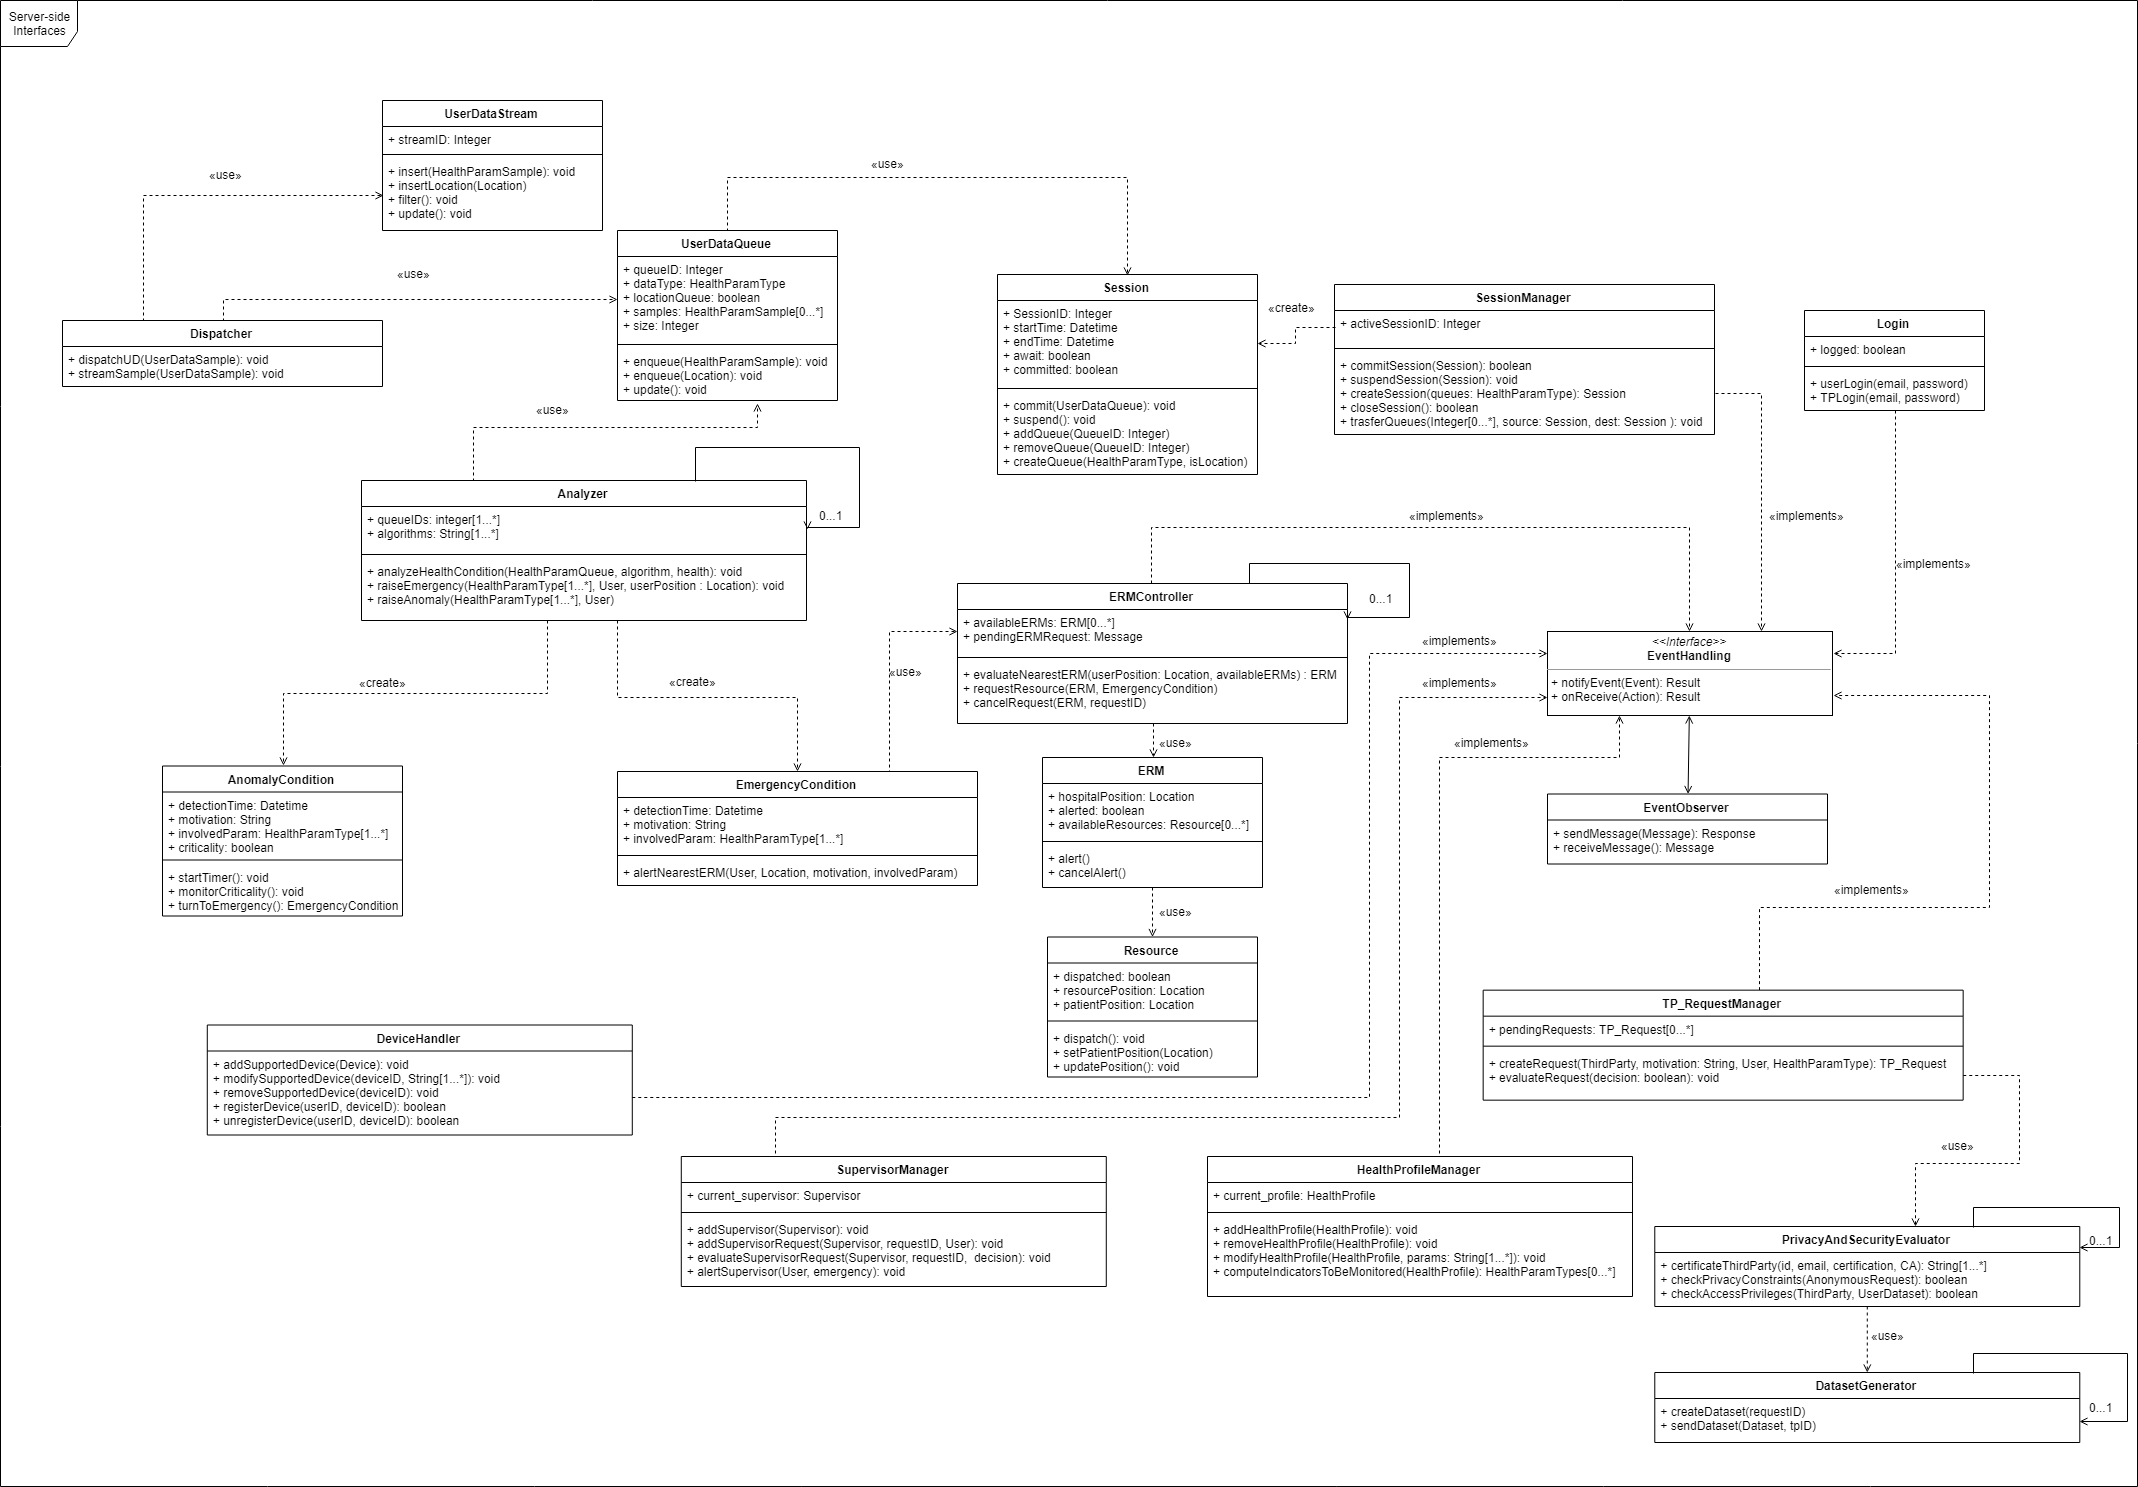
\includegraphics[scale=0.23]{images/uml/server_interfaces}
	\caption{Server Logic, Interface Dependencies}
	\label{Figure 16}
\end{figure}
\newpage


{\color{Blue}{\subsection{Selected Architectural Styles and Patterns}}}
{\setlength{\parskip}{0.3cm}
This part is dedicated to discuss about some design decision not explicitly represented in the rest of the document.
Several design patterns have been considered for both the architecture, in particular:
\begin{itemize}
	\item \textbf{Hardware Proxy Pattern}: that creates a software element responsible for access to a piece of hardware. It uses a class to encapsulate device information and all access to the hardware device, regardless of its physical interface;
	\item \textbf{Mediator Pattern}: to coordinate the interactions among different set of elements, a Mediator figure has been chosen. In particular, the best candidates, in this case, the \textit{EventObserver} and the \textit{EventHandling} interface have been conceived for allowing some components to notify events and perform specific operations when specific events occur, send and receive messages to and from the server, according to a predefined format;
	\item \textbf{Strategy Pattern}: since some components will implement different algorithms to perform specific tasks, this pattern has been chosen. To not complicate too much the UML diagrams and since many of this algorithms are not known at this stage of the development, the pattern has not been represented explicitly. However, the candidate classes are:
	\begin{itemize}
		\item \textbf{Analyzer}: different types of analysis following the same abstract model could be performed according to specific risk factors;
		\item \textbf{DataCollector}: that could collect data samples in many different ways from all the active devices.
	\end{itemize}
	\item \textbf{MVC (Model-View-Controller)}: at client side, this pattern allows separation between graphical representation of data, the business logic deployed to process it and data models;
	\item \textbf{Chain of Responsibility Pattern}: considered in the server architecture, in particular to:
	\begin{itemize}
		\item  regulate the interaction between the server and the ERMs for dispatching a rescue squad (Resource) when an emergency condition is detected. When the \textit{Analyzer} catches a dangerous situation, creates and delegates the responsibilities to alert the ERM to the \textit{EmergencyCondition} component, that, in turn, calls the \textit{ERMController} for alerting the hospital which is the nearest to the user;
		\item prevent third parties to access user datasets before allowing the system to certificate their identity and check the status of the relative request. The \textit{RequestManager} once ensured the second mentioned condition, delegates to the \textit{PrivacyAndSecurityEvaluator} the responsibilities to certificate the identity of the requester and to ensure that all the privacy constraints are respected by anonymous requests.
	\end{itemize} 
	\item \textbf{Singleton:} some classes, for several reasons (e.g: avoid resource access conflict) will be implemented as singleton (only the existance of a static instance is allowed)
\end{itemize}
}


{\color{Blue}{\subsection{Other Design Decisions}}}
On client side the defined architecture will interface with a little SQLite database hosted on the smartphone. It is well known how efficient SQLite Engine is, for smart embedded devices. Moreover, Android provides a full support in managing such database system in Android-based applications. In this document it is not explicitly inserted. After a team discussion, it has been decided to postpone the development of such part directly in the implementation stage. 

\end{flushleft}
